Considérons le dessin suivant, où les mesures des angles sont en radians.

\begin{center}
	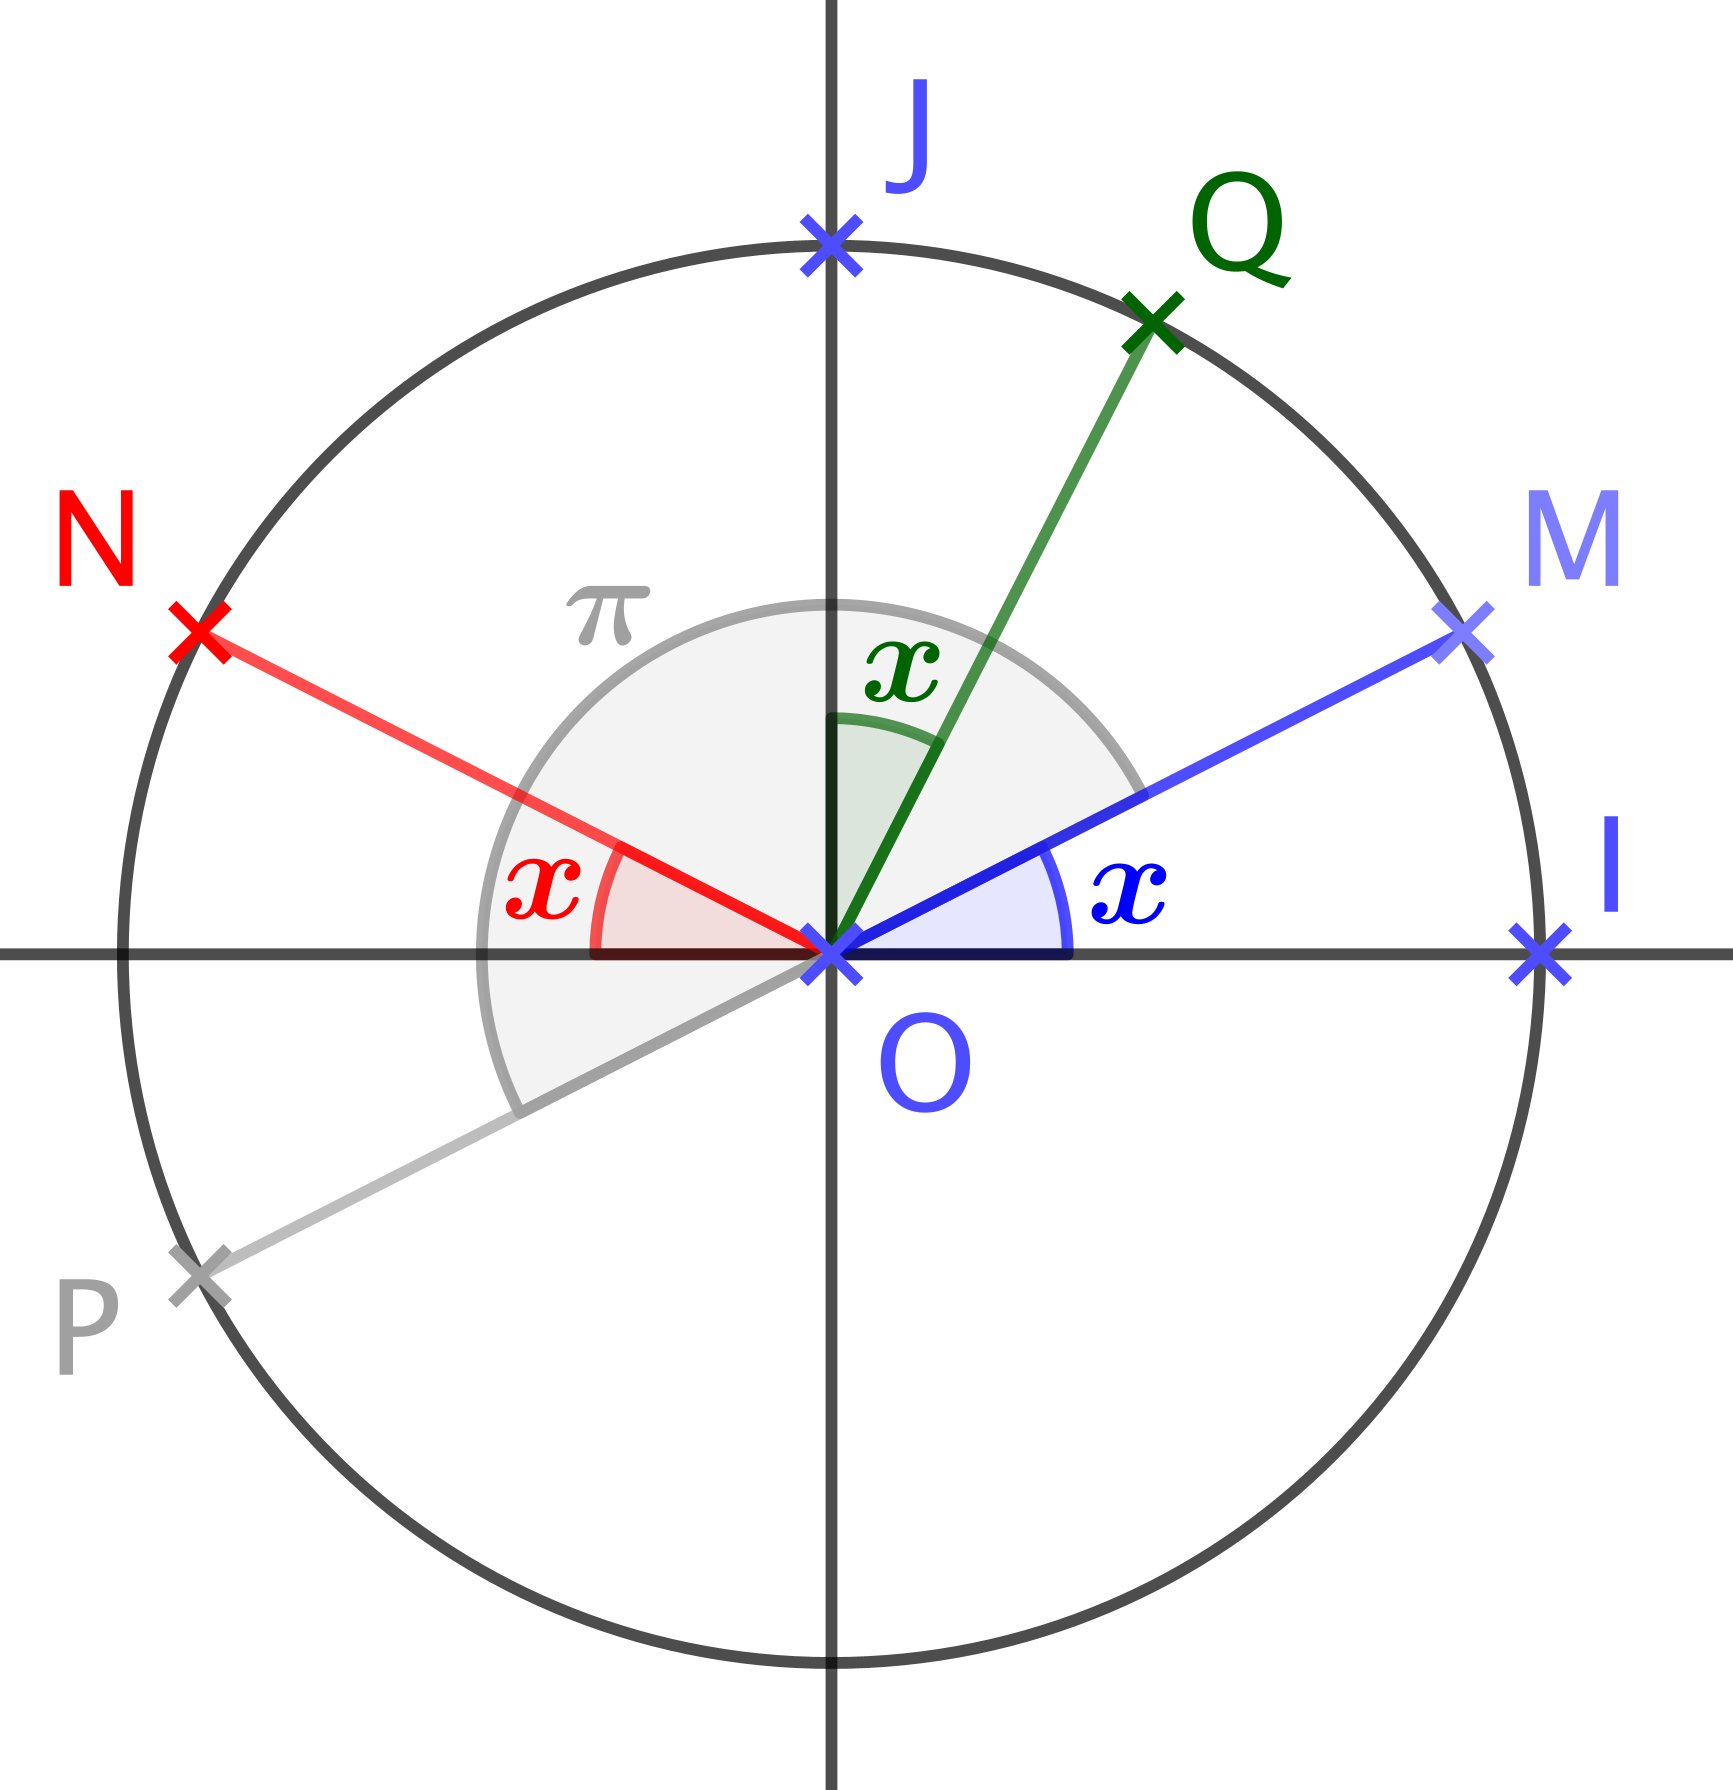
\includegraphics[scale = .7]{one-var-trig-formulas.png}
\end{center}

Via les points $M$, $N$, $P$ et $Q$, il est facile de fournir des arguments géométriques de symétrie justifiant que, sous la condition $x \in \intervalO{0}{\frac{\pi}{4}}$, nous avons:
%
\begin{multicols}{3}
\begin{itemize}[label=\small\textbullet]
	\item $\cos (\pi - x) = - \cos x$

	      \noindent
	      $\sin (\pi - x) = \sin x$ 

	\item $\cos (x + \pi) = - \cos x$

	      \noindent
	      $\sin (x + \pi) = - \sin x$

	\item $\cos \left( \frac{\pi}{2} - x \right) = \sin x$

	      \noindent
	      $\sin \left( \frac{\pi}{2} - x \right) = \cos x$ 
\end{itemize}
\end{multicols}


De nouveau, il serait bien de pouvoir passer, sans plus d'effort, à la validité des formules ci-dessus sur $\RR$ tout entier \emph{(considérer les autres cas n'est pas compliqué, mais c'est pénible)}.
%
Nous allons voir que cela est licite grâce au fait \ref{analytic-identity}, donné plus bas, qui est un peu technique, car il nécessite la notion de fonction analytique.


% ----------- %


\begin{preli} \label{conv-ray}
    Le rayon de convergence $R$ de la série entière complexe $\dsum_{n=0}^{\infty} a_n z^n$ est défini par la formule de Hadamard%
    \footnote{
    	La démonstration va révéler le côté \focus{naturel} de la formule de Hadamard.
    }
    $\displaystyle \frac{1}{R} = \limsup_{n \to +\infty} \big( \sqrt[n]{\abs{a_n}} \big)$
    avec les conventions
    $0 = \dfrac{1}{+\infty}$
    et
    $+\infty = \dfrac{1}{0}$.

    \smallskip
    
    Ce nombre $R$ s'interprète comme suit.
    \begin{enumerate}
        \item Si $R = 0$, la série ne converge que pour $z = 0$, et sinon elle diverge grossièrement.

        \item Si $R = +\infty$, la série converge sur $\CC$.
        Plus précisément, la série converge normalement sur tout disque ouvert $\CdiscO{0}{r}$ tel que $r \in \RRsp$. 

        \item Si $0 < R < +\infty$, la série converge normalement sur tout disque ouvert $\CdiscO{0}{r}$ tel que $0 < r < R$, donc elle converge sur $\CdiscO{0}{R}$.
        Par contre, elle diverge grossièrement sur $\CC - \CdiscC{0}{R}$,
        et
        le comportement sur le cercle $\Ccircle{0}{R}$ doit être traité au cas par cas.
    \end{enumerate}
\end{preli}


\begin{proof}
    Notons 
    $\displaystyle \ell
    = \limsup_{n \to +\infty} \big( \sqrt[n]{\abs{a_n}} \big)$,
    soit
    $\displaystyle \ell
    = \lim_{n \to +\infty} \big( \sup \big\{ \sqrt[k]{\abs{a_k}} \,,\, k \in \NN_{\geq n} \big\} \big)$,
    de sorte que $\ell \in \intervalC{0}{+\infty}$.
	%
    Commençons par le cas $\ell \in \RRsp$, c'est-à-dire $R \in \RRsp$.
    %
    \begin{itemize}
        \item Soit $r \in \intervalO{0}{R}$.
        %
        Considérons $\rho  \in \intervalO{r}{R}$ de sorte que $\frac1r > \frac{1}{\rho} > \frac1R$.
        Par définition de $\ell = \frac1R$,
        nous avons $n_0 \in \NN$ tel que
        $\sup \big\{ \sqrt[k]{\abs{a_k}} \,,\, k \in \NN_{\geq n_0} \big\} < \frac{1}{\rho}$.
        %
        Donc pour $z \in \CdiscO{0}{r}$ et $k \in \NN_{\geq n_0}$, nous obtenons
        $\abs{a_k z^k} < \big( \frac{r}{\rho} \big)^k$ pour $k \geq n_0$.
        Comme $0 < \frac{r}{\rho} < 1$, la convergence normale devient évidente.


        \item Soit $z \in \CC - \CdiscC{0}{R}$.
        %
        Comme $\frac{1}{\abs{z}} < \frac{1}{R}$, nous avons ici $n_0 \in \NN$ tel que
        $\forall n \in \NN_{\geq n_0}$,
        $\sup \big\{ \sqrt[k]{\abs{a_k}} \,,\, k \in \NN_{\geq n} \big\} > \frac{1}{\abs{z}}$.
        %
        En particulier,
        nous pouvons construire une suite strictement croissante d'indices $(k_i)$
        telle que
        $\abs{a_{k_i} z^{k_i}} > 1$.
        Ceci donne la divergence grossière.


        \item La justification du comportement pathologique sur le cercle $\Ccircle{0}{R}$ se fait via des contre-exemples. Nous pouvons citer les exemples classiques suivants.
        %
        \begin{enumerate}[label=(\alph*)]
	        \item $\dsum_{n=0}^{\infty} z^n$, 
	        de rayon de convergence $1$, 
	        diverge grossièrement sur $\Ccircle{0}{1}$.

	        \item $\dsum_{n=0}^{\infty} \frac{1}{n^2} z^n$, 
	        de rayon de convergence $1$,
	        puisque 
	        $ \ln \big( \sqrt[n]{\frac{1}{n^2}} \big)
	        = -\frac{2 \ln n}{n}$.
	        %
	        De plus,
	        cette série entière converge normalement sur $\Ccircle{0}{1}$.

	        \item $\dsum_{n=0}^{\infty}  \frac{1}{n} z^n$, 
	        de rayon de convergence $1$,
	        puisque 
	        $ \ln \big( \sqrt[n]{\frac{1}{n}} \big)
	        = -\frac{\ln n}{n}$.
	        %
	        De plus,
	        cette série entière converge sur $\Ccircle{0}{1} - \setgene{1}$, mais pas en $1$. 
	        Le comportement sur $\Ccircle{0}{1} - \setgene{1}$ est plus délicat à démontrer, car il se base sur le test de Abel-Dirichlet.
	    \end{enumerate}
    \end{itemize}


    Les cas
    $\ell = 0$, c'est-à-dire $R = +\infty$,
    et
    $\ell = +\infty$, c'est-à-dire $R = 0$,
    s'obtiennent via des adaptations immédiates de ce qui a été fait ci-dessus.
\end{proof}


\begin{example}
	La série entière complexe $\dsum_{n=0}^{\infty} \frac{1}{n!} z^n$ admet un rayon de convergence infini; la fonction associée est l'exponentielle complexe $\exp$.
	%
	En effet,
	notant $\ent$ la fonction partie entière, nous avons
	$n! \geq \big( \frac{n}{2} \big)^{\ent (\frac{n}{2})} \geq \big( \frac{n}{2} \big)^{\frac{n}{2} - 1}$,
	puis
	$ \ln \big( \sqrt[n]{\frac{1}{n!}} \big)
	\leq
	  \frac{2 - n}{2 n} \ln \big( \frac{n}{2} \big)$.
\end{example}


\begin{remark}
	On peut démontrer que
	$\exp : (\CC , {+}) \to (\CCs, {\times})$ est un morphisme de groupes, et que son noyau est du type $\ii r \ZZ$ avec $r \in \RRsp$.%
	\footnote{
	    Entre autres choses, ceci nécessite de savoir que
	    $f(z) = \exp z - 1$ n'a que des zéros isolés,
	    et
	    que les sous-groupes de $\RR$ sont soit denses, soit discrets et du type $r \ZZ$ avec $r \in \RRsp$. 
	}
	Posant $\pi = \frac{r}{2}$, le noyau s'écrit $2 \ii \pi \ZZ$.
	C'est un moyen, comme un autre, de définir et construire le nombre réel $\pi$.
\end{remark}


\begin{example} \label{cos-sin-analytic}
    Les fonctions circulaires sont définissables sur $\CC$ via
    $\cos z = \frac{\exp(\ii z) + \exp(- \ii z)}{2}$
    et
    $\sin z = \frac{\exp(\ii z) - \exp(- \ii z)}{2 \ii}$,
    c'est-à-dire via
    $\cos z = \dsum_{n=0}^{\infty} \frac{(-1)^n}{(2n)!} z^{2n}$
    et
    $\sin z = \dsum_{n=0}^{\infty} \frac{(-1)^n}{(2n+ 1)!} z^{2n+1}$.
    La remarque précédente donne la $2 \pi$-périodicité des fonctions complexes $\cos$ et $\sin$.
\end{example}


% ----------- %


\begin{preli} \label{der-power-serie}
    Soit une série entière complexe $\dsum_{n=0}^{\infty} a_n z^n$ de rayon de convergence $R$ non nul.
    %
    La fonction $f: z \in \CdiscO{0}{R} \mapsto \dsum_{n=0}^{\infty} a_n z^n \in \CC$ vérifie les propriétés suivantes.
    %
    \begin{enumerate}
    	\item $f$ est infiniment $\CC$-dérivable.%
		\footnote{
			L'analyse complexe étudie les fonctions $\CC$-dérivables en les nommant \focus{fonctions holomorphes}.
			Cette théorie est ludique, riche, et très utile.
		}

    	\item $\forall k \in \NN$,
		la série entière $\dsum_{n = k}^{\infty} \dfrac{n!}{(n-k)!} a_n z^{n - k}$ admet $R$ pour rayon de convergence.

    	\item $\forall k \in \NN$, $\forall z \in \CdiscO{0}{R}$,
		$\der[e]{f}{z}{k}(z) = \dsum_{n = k}^{\infty} \dfrac{n!}{(n-k)!} a_n z^{n - k}$.

    	\item \label{a_n-value}
		$\forall n \in \NN$,  $a_n = \dfrac{\der[e]{f}{z}{n}(0)}{n!}$.
    \end{enumerate}
\end{preli}


\begin{proof}
	La propriété \ref{a_n-value} étant aisée à déduire, une récurrence immédiate à faire montre qu'il suffit de démontrer que
	$\forall z \in \CdiscO{0}{R}$,
	$ \limit{\big( \frac{f(z) - f(z_0)}{z - z_0} \big)}%
	        {z}{z_0 | z \in \CdiscO{0}{R}}
	= \dsum_{n = 1}^{\infty} n a_n z^{n - 1}$.
	%
	\begin{itemize}
		\item
		$ \ln \big( \sqrt[n]{\abs{n a_n}} \big)
		= \frac{\ln n}{n} + \ln \big( \sqrt[n]{\abs{a_n}} \big)$
		donne que
		$R$ est le rayon de convergence de
		$\dsum_{n = 1}^{\infty} n a_n z^{n - 1}$.
		On peut donc définir la fonction $g: z \in \CdiscO{0}{R} \mapsto \dsum_{n = 1}^{\infty} n a_n z^{n - 1} \in \CC$.


		\item Pour $(z , z_0) \in \CdiscO{0}{R}^2$ et $k \in \NNs$, nous introduisons les notations suivantes.
        %
        \begin{enumerate}[label=(\alph*)]
	        \item $f_k(z) = \dsum_{n = 0}^{k} a_n z^n$.

	        \item $g_k(z) = \dsum_{n = 1}^{k} n a_n z^{n-1}$,
	        cette fonction étant clairement la $\CC$-dérivée de $f_k(z)$.

	        \item $T_k(z) =
			\begin{cases}
	    		  \frac{f_k(z) - f_k(z_0)}{z - z_0}
				& \text{si $z \in \CdiscO{0}{R} - \setgene{z_0}$}
				\\
	   			  g_k(z_0) 
				& \text{si $z = z_0$}
	 		\end{cases}$

	        \item $T(z) =
			\begin{cases}
	    		  \frac{f(z) - f(z_0)}{z - z_0} 
				& \text{si $z \in \CdiscO{0}{R} - \setgene{z_0}$}
				\\
	   			  g(z_0)
				& \text{si $z = z_0$}
	 		\end{cases}$
	    \end{enumerate}


		\item Considérons alors $r \in \intervalO{0}{R}$ tel que $z_0 \in \CdiscO{0}{r}$.
		Par convergence normale sur $\CdiscC{0}{r}$ de $(f_k)_k$ et $(g_k)_k$ vers $f$ et $g$ respectivement,
		nous avons la convergence uniforme sur $\CdiscC{0}{r}$ de $(T_k)_k$ vers $T$. 
		Or chaque fonction $T_k$ est continue en $z_0$ par $\CC$-dérivablité de $f_k$, donc $T$ est continue en $z_0$,
		d'où
		la $\CC$-dérivabilité de  $f$ en $z_0$ avec $\der{f}{z}{1}(z_0) = g(z_0)$.
		Ceci achève la preuve, car $z_0 \in \CdiscO{0}{R}$ est quelconque.
	\end{itemize}

	\null\vspace{-6ex}
\end{proof}


\begin{remark} \label{der-power-serie-gene}
	Une relecture de preuves des \refprelis{conv-ray} et \ref{der-power-serie} donnent que pour toute série entière complexe $\dsum_{n=0}^{\infty} a_n z^n$ de rayon de convergence $R$ non nul,
	et tout nombre complexe $z_0$,
	la fonction $f: z \in \CdiscO{z_0}{R} \mapsto \dsum_{n=0}^{\infty} a_n (z - z_0)^n \in \CC$ vérifie les propriétés suivantes.
    %
    \begin{enumerate}
    	\item $f$ est infiniment $\CC$-dérivable.

    	\item $\forall k \in \NN$,
		la série $\dsum_{n = k}^{\infty} \frac{n!}{(n-k)!} a_n (z - z_0)^{n - k}$ converge normalement sur $\CdiscO{z_0}{R}$,

    	\item $\forall k \in \NN$, $\forall z \in \CdiscO{z_0}{R}$,
		$\der[e]{f}{z}{k}(z) = \dsum_{n = k}^{\infty} \frac{n!}{(n-k)!} a_n (z - z_0)^{n - k}$.

    	\item $\forall n \in \NN$, $a_n = \frac{\der[e]{f}{z}{n}(z_0)}{n!}$.
    \end{enumerate}
\end{remark}


% ----------- %


Nous allons voir que les fonctions développables en série entière autour d'un nombre complexe $z_0$ ont le bon ton de l'être aussi dans un voisinage de $z_0$.


\begin{defi} \label{def-analytic}
    Soit $\Omega \subseteq \CC$ un ouvert non vide.
	%
	Une fonction $f: \Omega \rightarrow \CC$ est dite analytique en $z_0 \in \Omega$, 
	s'il existe
	une série entière $\dsum_{n = 0}^{+\infty} a_n z^n$
	de rayon de convergence $R > 0$
	et
	un réel $r \in \intervalOC{0}{R}$ tels qu'on ait
	$f(z) = \dsum_{n = 0}^{+\infty} a_n (z - z_0)^n$
	dans le disque ouvert $\CdiscO{z_0}{r} \subseteq \Omega$.

	\smallskip
	
	Si $f$ est analytique en tout nombre complexe de $\Omega$,
	la fonction $f$ est dite analytique sur $\Omega$.
\end{defi}


% ----------- %


\begin{fact} \label{power-serie-vs-analytic}
    Soit $f: \Omega \rightarrow \CC$ où $\Omega \subseteq \CC$ est un ouvert non vide.
    %
    Si $f$ est analytique en $z_0$,
	alors
	il existe un réel $r > 0$ tel que $f$ soit analytique sur $\CdiscO{z_0}{r}$ tout entier. 
\end{fact}


\begin{proof}
    Reprenons les notations de la \refdefi{def-analytic}.
    Nous allons montrer que le réel $r$ convient.
    Pour cela, considérons $\omega \in \CdiscO{z_0}{r}$
    et
    un disque ouvert non vide $\CdiscO{\omega}{\rho} \subseteq \CdiscO{z_0}{r}$.
    Notons que $0 < \rho < r$.
	%
	\begin{itemize}
		\item Formellement,
		$f(z) = \dsum_{n = 0}^{\infty} \frac{\der[e]{f}{z}{n}(\omega)}{n!} (z - \omega)^n$
		et
		$\der[e]{f}{z}{n}(\omega) = \dsum_{k = n}^{\infty} \frac{k!}{(k-n)!} a_k \omega^{k - n}$
		conduisent à étudier
		$ \dsum_{n = 0}^{\infty} \dsum_{k = n}^{\infty} \frac{k!}{n! (k-n)!} a_k \omega^{k - n} (z - \omega)^n
		= \dsum_{n = 0}^{\infty} \dsum_{q = 0}^{\infty} \frac{(n+q)!}{n! q!} a_{n+q} \omega^q (z - \omega)^n$.
	

		\item Soit $F \subset \NN^2$ un ensemble fini.
		%
		Introduisons les notations suivantes.
		%
		\begin{enumerate}
			\item $\sigma_F(z ; \omega) = \dsum_{(n,q) \in F} \alpha_{n,q}(z ; \omega)$
			où
			$\alpha_{n,q}(z ; \omega) = \frac{(n+q)!}{n! q!} a_{n+q} \omega^q (z - \omega)^n$.

			\item $\mu(z) = \dsum_{n = 0}^{+\infty} \abs{a_n} z^n$ qui est de rayon de convergence $R$.

			\item $N = \max \big\{ n + q \,,\, (n,q) \in F \big\}$.
		\end{enumerate}
		
		\noindent
		Pour $z \in \CdiscO{\omega}{\rho}$, nous avons:
		
		\noindent\kern-6pt
		\begin{stepcalc}[style=sar, ope=\leq]
			\dsum_{(n,q) \in F} \abs{\alpha_{n,q}(z ; \omega)}
		\explnext{}
			\dsum_{s=0}^{N} \dsum_{n+q=s} \abs{\alpha_{n,q}(z ; \omega)}
		\explnext{}
			\dsum_{s=0}^{N} \dsum_{n+q=s} \binom{n+q}{q} \abs{a_{n+q}} r^q \rho^n
		\explnext{}
			\dsum_{s=0}^{N} \abs{a_s} \big( \dsum_{n+q=s} \binom{n+q}{q} r^q \rho^n \big)
		\explnext{}
			\dsum_{s=0}^{N} \abs{a_s} (r + \rho)^s
		\explnext{}
			\dsum_{s=0}^{+\infty} \abs{a_s} (r + \rho)^s
		\end{stepcalc}
		
		\noindent
		En imposant $r + \rho < R$, c'est-à-dire $\rho < R - r$, 
		pour tout sous-ensemble fini $F$ de $\NN^2$, nous avons
		$\dsum_{(n,q) \in F} \abs{\alpha_{n,q}(z ; \omega)} \leq \mu(r + \rho) < +\infty$.
		
		\noindent
		Donc
		$\dsum_{(n,q) \in \NN^2} \alpha_{n,q}(z ; \omega)$
		est absolument convergente,
		et commutativement convergente.
	

		\item Pour $z \in \CdiscO{\omega}{\rho} \subseteq \CdiscO{z_0}{r}$, où $0 < \rho < R - r$, ce qui suit nous donne, comme souhaité,
		$f(z) = \dsum_{n = 0}^{\infty} \frac{\der[e]{f}{z}{n}(\omega)}{n!} (z - \omega)^n$.

        \begin{multicols}{2}
        	\begin{enumerate}[wide]
    			\item
        		\begin{stepcalc}[style=ar*]
        			\dsum_{(n,q) \in \NN^2} \alpha_{n,q}(z ; \omega)
        		\explnext{}
        			\dsum_{s=0}^{+\infty} \dsum_{n+q=s} \alpha_{n,q}(z ; \omega)
        		\explnext{}
        			\dsum_{s=0}^{+\infty} \dsum_{n+q=s} \binom{n+q}{q} a_{n+q} \omega^q (z - \omega)^n
        		\explnext{}
        			\dsum_{s=0}^{+\infty} a_s \big( \dsum_{n+q=s} \binom{n+q}{q} \omega^q (z - \omega)^n \big)
        		\explnext{}
        			\dsum_{s=0}^{+\infty} a_s (\omega + z - \omega)^s
        		\explnext{}
        			f(z)
        		\end{stepcalc}


    			\item
        		\begin{stepcalc}[style=ar*]
        			\dsum_{(n,q) \in \NN^2} \alpha_{n,q}(z ; \omega)
        		\explnext{}
        			\dsum_{n = 0}^{\infty} \dsum_{q = 0}^{\infty} \alpha_{n,q}(z ; \omega)
        		\explnext{}
        			\dsum_{n = 0}^{\infty} \dsum_{q = 0}^{\infty} \binom{n+q}{q} a_{n+q} \omega^q (z - \omega)^n
        		\explnext{}
        			\dsum_{n = 0}^{\infty} \dsum_{k = n}^{\infty} \binom{k}{k-n} a_{k} \omega^{k-n} (z - \omega)^n
        		\explnext{}
        			\dsum_{n = 0}^{\infty} \frac{1}{n!} (z - \omega)^n \big( \dsum_{k = n}^{\infty} \frac{k!}{(k-n)!} a_{k} \omega^{k-n} \big) 
        		\explnext{}
        			\dsum_{n = 0}^{\infty} \frac{\der[e]{f}{z}{n}(\omega)}{n!} (z - \omega)^n
        		\end{stepcalc}
    		\end{enumerate}
	\end{multicols}
	\end{itemize}

	\null\vspace{-8ex}
\end{proof}


% ----------- %


Passons, enfin, au résultat essentiel de cette section qui va permettre de valider nos identités trigonométriques obtenues partiellement via la géométrie.


\begin{fact} \label{isolated-zero}
    Soit $\Omega \subseteq \CC$ un ouvert connexe non vide,%
    \footnote{
    	On parle aussi de \focus{domaine complexe}.
    }
    et
    $f: \Omega \rightarrow \CC$ une fonction analytique non identiquement nulle.
    %
	Pour tout zéro $\alpha$ de $f$, il existe un disque ouvert non vide $\CdiscO{\alpha}{r} \subseteq \Omega$ tel que 
	$\forall z \in \CdiscO{\alpha}{r} - \setgene{\alpha}$, $f(z) \neq 0$
	\emph{(c'est le principe des zéros isolés)}.  
\end{fact}


\begin{proof}
	Nous allons voir que la connexité est essentielle. Rappelons que ceci signifie que $\emptyset$ et $\Omega$ sont les seules sous-ensembles de $\Omega$ qui sont à la fois ouverts et fermés.
	
	\smallskip
	
	$\forall \omega \in \Omega$, il existe un disque ouvert $\CdiscO{\omega}{r} \subseteq \Omega$ sur lequel 
	$f(z) = \dsum_{n = 0}^{\infty} \frac{\der[e]{f}{z}{n}(\omega)}{n!} (z - \omega)^n$.
	%
	Ceci permet de constater que les deux ensembles suivants sont identiques.
	%
	\begin{enumerate}
		\item $V = \setgene{\omega \in \Omega \mid \text{$f$ s'annule sur un voisinage de $\omega$}}$

		\item $D = \setgene{\omega \in \Omega \mid \forall n \in \NN, \der[e]{f}{z}{n}(\omega) = 0}$
	\end{enumerate}
		
	Clairement,
	$V$ est ouvert, et $D$ fermé, donc, par raison de connexité, $D$ est soit vide, soit égal à $\Omega$.
	Comme $f$ n'est pas identiquement nulle sur $\Omega$, seule l'alternative $D = \emptyset$ est possible.

	\smallskip
	
	Supposons alors avoir un zéro $\alpha$ de $f$. Le point précédent donne $m \in \NNs$ tel que 
	$\forall n \in \ZintervalCO{0}{m}$, $\der[e]{f}{z}{n}(\alpha) = 0$,
	et
	$\der[e]{f}{z}{m}(\alpha) \neq 0$.
	Ceci permet d'écrire
	$f(z) = (z - \alpha)^m \dsum_{n = m}^{\infty} a_n (z - \alpha)^{n - m}$
	sur un disque ouvert non vide $\CdiscO{\alpha}{\rho} \subseteq \Omega$,
	avec $a_m = \frac{\der[e]{f}{z}{m}(\alpha)}{m!} \neq 0$.
	Posant $g(z) = \dsum_{n = m}^{\infty} a_n (z - \alpha)^{n - m}$, nous obtenons une fonction continue sur $\CdiscO{\alpha}{\rho}$, et vérifiant $g(\alpha) \neq 0$.
	Comme $f(z) = (z - \alpha)^m g(z)$, il devient clair qu'il existe $r > 0$ tel que
	$\CdiscO{\alpha}{r} \subseteq \CdiscO{\alpha}{\rho}$
	et
	$\forall z \in \CdiscO{\alpha}{r} - \setgene{\alpha}$, $f(z) \neq 0$.
\end{proof}


% ----------- %

\begin{example}
    Notre raisonnement géométrique de début de section fait clairement apparaître des zéros non isolés pour les fonctions analytiques sur $\CC$ suivantes, l'analycité des $f_k$ venant de celle des fonctions complexes $\cos$ et $\sin$ (voir l'\refexa{cos-sin-analytic}).
    %
    \begin{itemize}[label=\small\textbullet]
    	\item $f_1(z) = \cos (\pi - z) + \cos z$ 
    	   et $f_2(z) = \sin (\pi - z) - \sin z$ 
    
    	\smallskip
    	\item $f_3(z) =\cos (z + \pi) + \cos z$ 
    	   et $f_4(z) =\sin (z + \pi) + \sin z$
    
    	\smallskip
    	\item $f_5(z) =\cos \left( \frac{\pi}{2} - z \right) - \sin z$ 
    	   et $f_6(z) =\sin \left( \frac{\pi}{2} - z \right) - \cos z$ 
    \end{itemize}
\end{example}
